\chapter{Einleitung}
\section{Motivation}
\label{sec:motivation}
Motiviert wurde diese Arbeit durch den Artikel \cite{doi:10.1021/acsnano.1c00139}, aus welchem jegliche Informationen dieses 
Abschnitts entnommen wurden.
In dem dort behandelten Experiment wird mittels ultra-niederenergetischer Ionenimplantation
(\textit{ultralow-energy ion implantation}) Mangan (Mn) in eine einzelne Graphenstörstelle, wobei sich das Graphen auf einem Kupfersubstrat befindet, eingesetzt.
Es wurden die Positionen des Mn im Bezug auf die Moiré Superstruktur (Abbildung \ref{fig:ascnano_structure}), die elektronischen und magnetischen Eigenschaften und die Konzentration der Mn-Defekte
untersucht.
Die Moiré Superstruktur bildet sich aus, da die vertikale Ausrichtung zwischen dem Graphen und dem Kupfer kontinuierlich variiert.
\begin{figure}[H]
    \centering
    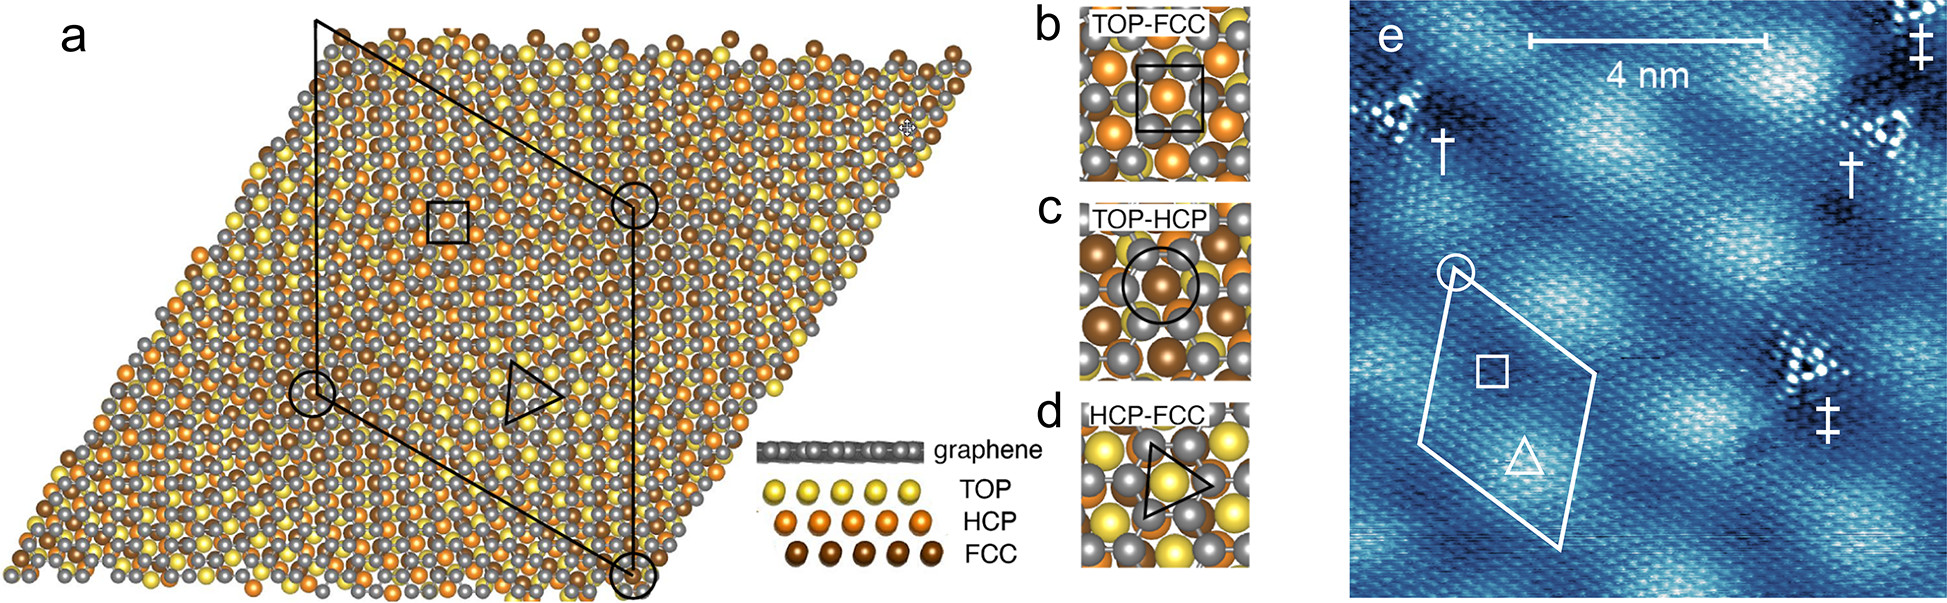
\includegraphics[width = \textwidth]{Plots/images_large_nn1c00139_0002.jpeg}
    \caption{(a) zeigt die Moiré Superstruktur. Durch kontinuierliche Variation der der Ausrichtung 
    zwischen dem Kupfer und Graphen, entstehen Hochsymmetriepunkte bezüglich des Stapelns (b-d).
    Diese Hochsymmetriepunkte und somit auch die Moiré Superstruktur können mittels Rastertunnelmikroskopie (RTM) 
    visualisiert werden, womit eine zweidimensionale Periodizität ersichtlich wird (e).
    (Abbildung entnommen  aus \cite{doi:10.1021/acsnano.1c00139})}
    \label{fig:ascnano_structure}
\end{figure}
Graphen mit Mn-Störstellen eignet sich für die Untersuchung elektrischer und magnetischer Eigenschaften, da die Bänder bei einer Konzentration von ca. $\qty{0.04}{\percent}$ 
die Dirac-Eigenschaften beibehalten und es somit ein ideales System für das Studieren der Interaktion
zwischen lokalen magnetischen Momenten und den Dirac-Elektronen (siehe Abschnitt \ref{sec:propertiesofgraphene})darstellt.
Abbildung \ref{fig:ascnano_structure}a zeigt die Probe auf atomarer Ebene, worin auch die Moiré Superstruktur deutlich wird.
Die Stellen mit hoher Symmetrie bezüglich des Stapelns des Graphens auf dem Substrat werden in 
Abbildung \ref{fig:ascnano_structure}b-d aufgezeigt.
Diese bilden wiederrum ein zweidimensionales Gitter (Abb. \ref{fig:ascnano_structure}e).
Aufgrund der kurzen Reichweite der Bindungen, welche Graphen charakterisiert, und des großen Radius von Mn im Vergleich zur 
Kohlenstofffehlstelle entweicht das Mn senkrecht zur Graphenebene.
Dieses kann sich zwischen das Graphen und das Substrat oder zwischen Graphen und Vakuum (nach außen gerichtet) entweichen. 
Jedoch wurden mögliche nach außen gerichtete Anordnung nur mit einer Wahrscheinlichkeit, 
welche um mehr als zwei Größenordnungen kleiner ist, beobachtet.
Dies liegt daran, dass die Konfiguration mit dem nach außen gerichteten Mn eine höhere Energie aufweist und somit instabiler ist.
Während das Mn zum Kupfersubstrat entweicht, nehmen die Kohlenstoffatome um diese Störstelle herum eine nach außen gerichtete Positon ein.
\begin{figure}
    \centering
    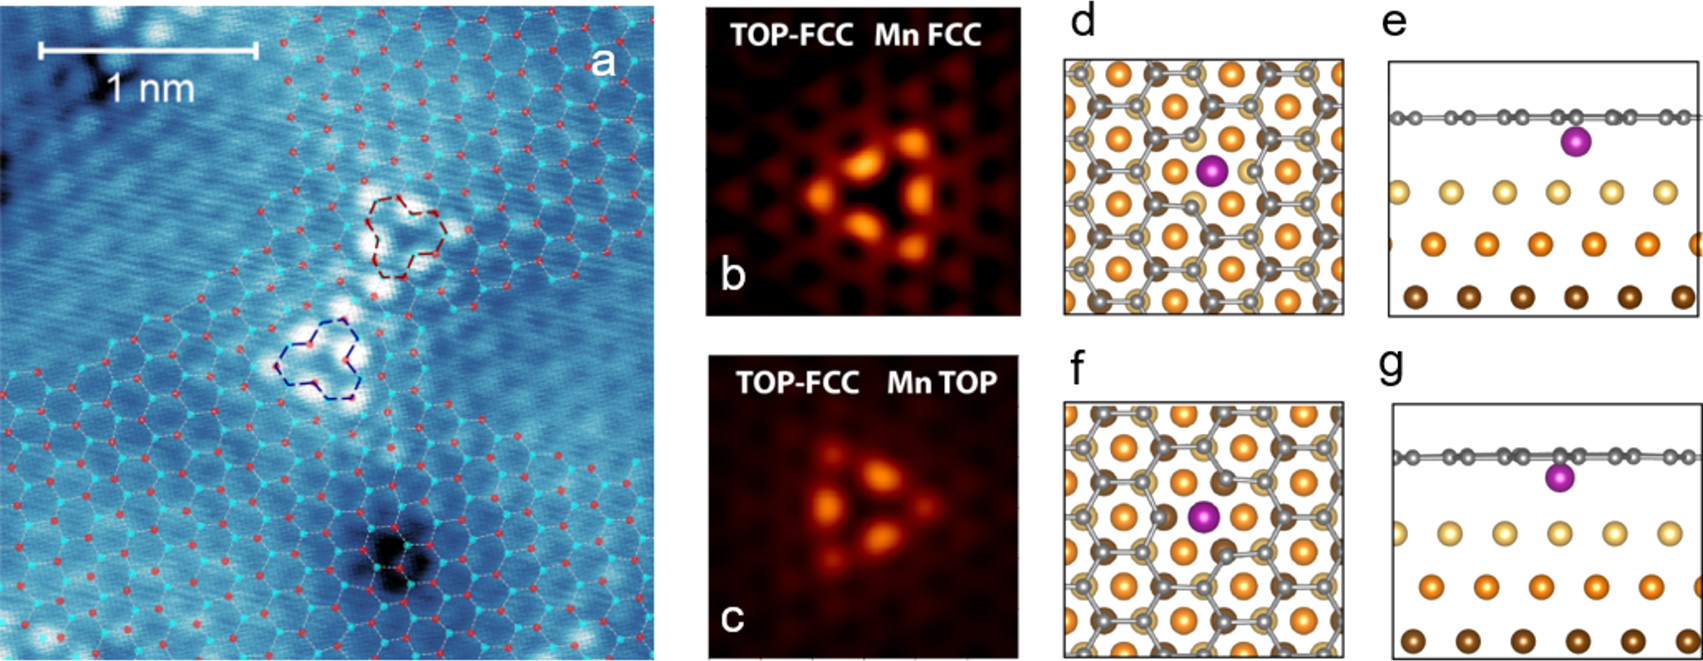
\includegraphics[width = \textwidth]{Plots/images_large_nn1c00139_0003.jpeg}
    \caption{(a) zeigt eine RTM, in welcher ersichtlich wird, dass Mn in die beiden verschiedenen Untergittern von Graphen implantiert wurde. In der
    RTM äußern sich diese mittels dreieckigen Strukturen, welche zueinander gespiegelt liegen.
    (b-c) zeigen RTM simuliert mittels Dichtefunktionaltheorie (DFT) in einer TOP-FCC Region. In (b) liegt das Mn auf einem FCC
    und in (c) auf einem TOP Gitterplatz. (d,e) zeigt das Mn auf einem FCC und (f,g) zeigt es auf einem TOP Platz in der Graphenebene und seitlich davon.
    (Abbildung entnommen  aus \cite{doi:10.1021/acsnano.1c00139})}
    \label{fig:ascnano_defect}
\end{figure}
Für die sechs verschiedenen Plätze des Mn (zwei Untergitter und drei Hochsymmetrieregionen) wurden DFT-Rechnungen für die Energien und die magnetischen Momente gemacht.
Dabei zeigte sich, dass diese Größen von dem lokalen Stapeln und dem Untergitter abhängen, so dass die Energie geringer ist, womit 
diese Konfiguration (z.B. Mn auf einem FCC PLatz in einer TOP-FCC-Region) höhere Stabilität aufweist.
Dies Tendenz zeigte sich ebenfalls in den RTM, wobei angemerkt werden muss, dass die Datenlage dazu nicht ausreicht, um
verlässliche Ergebnisse zu haben.  
\newpage
\FloatBarrier
\section{Struktur von Graphen und der Störstelle}
\label{sec:structure}
\begin{wrapfigure}{r}{0.49\textwidth}
    \centering
    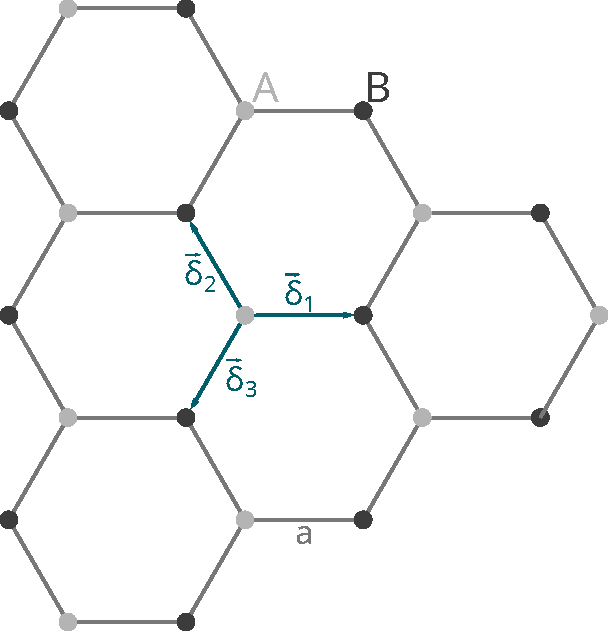
\includegraphics[width = 0.49\textwidth]{Plots/graphene_lattice.pdf}
    \caption{Das für Graphen typische Honigwabengitter. Die Kristallstruktur wird durch zwei Untergitter (A und B) und den 
    Gittervektoren $\vec{a}_1$ und $\vec{a}_2$ beschrieben, wobei
    die drei nächsten Nachbarn, die einen Abstand von $a$ (Gitterkonstante) haben, die Abstandsvektoren $\vec{\delta}_i$ besitzen.}
    \label{fig:graphene_lattice}
\end{wrapfigure}
Graphen ist ein zweidimensionales, aus einer Atomschicht bestehendes Allotrop von Kohlenstoff, dessen
Struktur nur mit einer zweiatomigen Basis (Atom A und B) beschrieben werden kann, da sonst keine Translationsinvarianz vorherrschen würde.
Wird mit diesen inäquivalenten Atomen eine Basis gebildet, ergibt sich mit den Gittervektoren 
\begin{equation*}
        \vec{a}_1 = \frac{a}{2}\begin{pmatrix} 3 \\[4pt] \sqrt{3}  \end{pmatrix}, \quad
        \vec{a}_2 = \frac{a}{2}\begin{pmatrix} 3 \\[4pt] -\sqrt{3} \end{pmatrix}       
\end{equation*}    
ein zweidimensionales, hexagonales Gitter.
Die Abstandsvektoren $\vec{\delta}_i(\varphi_i)$ der drei benachbarten B-Atome eines A-Atoms können mit Hilfe eines 
diskreten Drehwinkels $\varphi_i \in \{ 0,  \sfrac{2\pi}{3}, \, \sfrac{4\pi}{3} \} $ angegeben werden (Abb. \ref{fig:graphene_lattice}), so dass sich $a$ als Gitterabstand
$\vec{\delta}_i(\varphi_i) = a \, ( \sin (\varphi_i), \cos (\varphi_i) )$
ergibt.
Bei Betrachtung von drei um ein B-Atom umliegenden A-Atomen sind die Abstandsvektoren gespiegelt.
Das Koordinatensystem kann so gelegt werden, so dass $\vec{\delta}_1$ auf der x-Achse liegt, womit sich die Abstandsvektoren mittels
\begin{equation*}
    \vec{\delta}_1 = a \begin{pmatrix} 1            \\[4pt] 0                   \end{pmatrix}, \quad
    \vec{\delta}_2 = a \begin{pmatrix} -\frac{1}{2} \\[4pt] \frac{\sqrt{3}}{2}  \end{pmatrix}, \quad 
    \vec{\delta}_3 = a \begin{pmatrix} -\frac{1}{2} \\[4pt] -\frac{\sqrt{3}}{2} \end{pmatrix}
\end{equation*}
darstellen lassen.
Wird nun ohne Beschränkung der Allgemeinheit ein Kohlenstoffatom aus dem Untergitter A entfernt und dort Mn eingesetzt (Abb. \ref{fig:mangan_impurity_inplane}), 
ändern sich die Abstandsvektoren. 
Dies liegt, wie im vorigen Abschnitt \ref{sec:motivation} diskutiert, daran, dass das Manganatom zu groß ist und nicht in diese Stelle passt, so dass es aus der Ebene entweicht und 
eine $z$-Komponente besitzt.
Diese Situation ist in Abbildung \ref{fig:mangan_impurity} dargestellt.
Die hinzukommende $z$-Komponente lässt sich mittels trigonometrischen Beziehungen zu $z = -\cot (\theta)$ bestimmen, womit die 
Abstandsvektoren durch 
\begin{equation*}
    \vec{d}_1 = a \begin{pmatrix} 1            \\[4pt] 0                   \\[4pt] \cot (\theta)\end{pmatrix}, \quad
    \vec{d}_2 = a \begin{pmatrix} -\frac{1}{2} \\[4pt] \frac{\sqrt{3}}{2}  \\[4pt] \cot (\theta)\end{pmatrix}, \quad 
    \vec{d}_3 = a \begin{pmatrix} -\frac{1}{2} \\[4pt] -\frac{\sqrt{3}}{2} \\[4pt] \cot (\theta)\end{pmatrix}
\end{equation*}
angegeben werden können.
Wie bereits in Abbildung \ref{fig:mangan_impurity} angedeutet, wird im Folgenden angenommen, dass das Mn mittig von den nächsten Nachbarn liegt, so dass 
sich die $x$- und $y$-Komponente der Abstandsvektoren nicht ändert.
\begin{figure}
    \begin{subfigure}{0.48\textwidth}%
    \centering%
    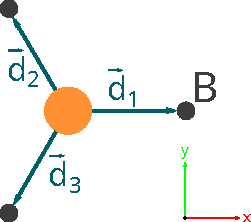
\includegraphics[height = 2.8cm]{Plots/mangan_impurity_inplane.pdf}%
    \caption{Mn-Störstelle in der Graphenebene.}%
    \label{fig:mangan_impurity_inplane}%
    \end{subfigure}%
    \hfill% Fills available space in the center -> space between figures
    \begin{subfigure}{0.48\textwidth}%
    \centering%
    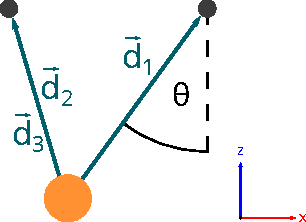
\includegraphics[height = 2.8cm]{Plots/mangan_impurity_z_component.pdf}%
    \caption{Mn-Defekt in einer seitlichen Ansicht.}%
    \label{fig:mangan_impurity_z_component}%
    \end{subfigure}%
    \caption{Darstellung des räumlichen Anordnung des Mangandefekts aus veschiedenen Ansichten.
    Aus dem Untergitter A wurde ein Kohlenstoffatom entfernt und Mangan (orange) implantiert.
    Wie in Abschnitt \ref{sec:motivation} diskutiert, entweicht das Mn aus der Graphenebene.}%
    \label{fig:mangan_impurity}%
\end{figure}%
Hierbei ist es irrelevant, ob eine positive oder negative $z$-Komponente gewählt wird, da die Anordnung ohne Betrachtung des Kupfersubstrats 
spiegelsymmetrisch um die Graphenebene ist. 
Die $z$-Komponente wird negativ gewählt, damit dies konsistent mit dem Experiment ist.
Um die Bandstruktur beschreiben zu können, wird das reziproke Gitter, 
dessen Form ein um $\ang{90;;}$ gedrehtes Hexagon ist, benötigt \cite{honey}.
Dazu ist in Abbildung \ref{fig:first-brillouine-zone} die Erste Brillouin-Zone mit den 
reziproken Gittervektoren (Berechung im Anhang \ref{sec:rez_lattivectors_calc})
\begin{equation*}
    \vec{b}_1 = \frac{2\pi}{3a} \begin{pmatrix}  1\\[4pt]   \sqrt{3}  \end{pmatrix}, \quad
    \vec{b}_2 = \frac{2\pi}{3a} \begin{pmatrix}  1\\[4pt] - \sqrt{3} \end{pmatrix}       
\end{equation*}    
aufgezeigt.
\begin{wrapfigure}{l}{0.4\textwidth}
    \centering
    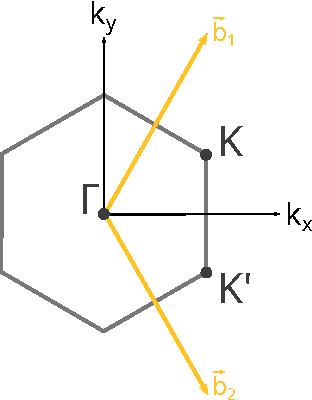
\includegraphics[width = 0.3\textwidth]{Plots/graphene_first_brillouine_zone.pdf}
    \caption{Erste Brillouin-Zone von Graphen.
    Eingezeichnet sind die reziproken Gittervektoren $\vec{b}_1$ und $\vec{b}_2$.
    Der $\symup{\Gamma}$-Punkt (Mitte der ersten Brillouine-Zone) und die beiden inäquivalenten
    Eckpunkte K und K$'$.}
    \label{fig:first-brillouine-zone}
\end{wrapfigure}
Besonders die Eckpunkte, $\vec{K} = \sfrac{2\pi}{3\sqrt{3}a} \, (\sqrt{3},1)$ 
und $\vec{K}' = \sfrac{2\pi}{3\sqrt{3}a} \, (\sqrt{3},-1)$, sind von hoher Relevanz, wie sich im folgenden Abschnitt herrausstellt.
In dieser Modellierung wird davon ausgegangen, dass Graphen komplett eben ist. 
In der Realität ist dem nicht so, da dem Mermin-Wagner Theorem nach langwellige Fluktuationen die reichtweitige Ordnung von zweidimensionalen Kristallen zerstören, womit
diese eine Krümmung aufweisen \cite{Fasolino2007}.
\FloatBarrier
\section{Eigenschaften von Graphen}
\label{sec:propertiesofgraphene}
Der größte Teil der Bindungen von Graphen geht von den $sp^2$-Hybridorbitalen aus, mit welcher ein Kohlenstoffatom mit drei umliegenden
Nachbarn in trigonalen und planaren Anordnung eine $\sigma$-Bindung eingeht \cite{RevModPhys.81.109}.
Das dazu senkrecht stehende $p$-Orbital führt zu einer weiteren Bindung, der $\pi$-Bindung, so dass ein Kohlenstoffatom
mit einem der drei nächsten Nachbarn eine Doppelbindung eingeht.
Dabei sorgt das $\sigma$-Band für die Robustheit der Gitterstruktur \cite{RevModPhys.81.109}.
Aufgrund des Pauli-Prinzips haben diese Bänder eine volle Schale, welche somit ein sehr tiefes Valenzband
formen \cite{RevModPhys.81.109}.
Da jedes $p$-Orbital, welches senkrecht auf der Graphenebene steht, ein Elektron
besitzt, ist das $\pi$-Band halb gefüllt, womit sich die Elektronen frei bewegen können \cite{RevModPhys.81.109}\cite{graphene_properties}.
Dieses $\pi$-Band trägt auch mit sehr großem Anteil zu der Leitfähigkeit von Graphen bei \cite{graphene_properties}.
Die Bandstruktur kann mittels einem Tight-Binding-Modell ermittelt werden, woraus unter der Annahme eines nächsten-Nachbarn-Hüpfens
die Dispersionsrelation 
\begin{equation*}
    \epsilon_{\vec{k}} \propto \pm \sqrt{3+2 \cos \left ( \sqrt{3}ak_y \right )+2\cos \left ( \frac{3}{2}ak_x+\frac{\sqrt{3}}{2}ak_y \right ) + 2\cos \left ( \frac{3}{2}ak_x-\frac{\sqrt{3}}{2}ak_y \right ) }
\end{equation*}
folgt (die Rechung dazu befindet sich im Anhang \ref{sec:calc_dispersion}).
Das negative bzw. positive Vorzeichen gehört zu dem Valenz- ($\pi$) bzw. Leitungsband ($\pi^*$) \cite{RevModPhys.81.109}.
Das Valenz- und Leitungsband berühren sich in zwei inäquivalenten Punkten der ersten Brillouin-Zone K und $\text{K}'$, welche 
auch Dirac-Punkte genannt werden \cite{10.1093/nsr/nwu080}.
Wird die Dispersionsrelation um diese beiden Punkte entwickelt, nimmt die Dispersionsrelationrelation eine lineare Form an, welche mit 
\begin{equation}
    \epsilon_{\vec{k}} \propto \pm | \vec{k} | 
\end{equation}
in der Nähe der beiden Punkte die Form eines Kegels (sog. \textit{Dirac cone}) besitzt \cite{10.1093/nsr/nwu080}\cite{Avouris2007}.
Jedoch verschwindet die Zustandsdichte in diesen Punkten, wodurch Graphen als ein bandlückenloser Halbleiter mit einer verschwindenen 
Zustandsdichte am Fermi-Niveau gesehen werden kann \cite{10.1093/nsr/nwu080}. 
Aufgrund dieser linearen Dispersion können die Elektronen durch die masselose Dirac-Gleichung beschrieben werden, wobei sich 
die Elektronen (in dem Fall sog. Dirac-Elektronen) mit der Fermigeschwindigkeit $v_\text{F}$ statt der Lichtgeschwindigkeit $c$ fortbewegen,
dessen Verhältnis $\sfrac{v_\text{F}}{c} \approx \sfrac{1}{300}$ ist \cite{Avouris2007}.
Dies führt zu einer sehr hohen Ladungsträgerbeweglichkeit \cite{https://doi.org/10.1002/adma.201201482}.
Graphen ist ebenfalls aufgrund dessen makroskopischen Eigenschaften von großem Interesse und ein aktuelles Forschungsthema.
Einerseits ist die  Dichte mit $\qty{0.77}{\milli\gram\per\metre\squared}$ extrem gering, obwohl 
Graphen eine hundertfache Stärke von Stahl bei der selben Dicke aufweist \cite{graphene_properties}. 
Anderseits ist Graphen das bisher bekannte, am besten leitende Material bei Raumtemperetur mit einer Leitfähigkeit von 
$\qty{e6}{\siemens\per\metre}$ \cite{graphene_properties}.